\documentclass{../source/Experiment}

\major{信息工程}
\name{姚桂涛}
\title{网页安全色}
\stuid{3190105597}
\college{信息与电子工程学院}
\date{\today}
\lab{}
\course{数字图像处理}
\instructor{李东晓}
\grades{}
\expname{网页安全色}
\exptype{设计验证}
\partner{}
\begin{document}
    \makecover
    \section{实验任务}
        本次选择的是PROJECT-06-01题目。
    

        \begin{enumerate}
            \item 编写一个程序将一个任意的RGB图像转换为一个网页安全色RGB图像。
            \item 下载Fif.6.8,并应用你写的程序将其转换为网页安全色,并解释你的结果和Fig.6.8的差异。
        \end{enumerate}
    \section{算法设计}
        
        网页安全色中RBG每一个部分的值只能是0,51,102,153,204,255这六个值,所以我将输入的RGB图像的每个部分的值按照0,51,102,153,204,255这进行量化,从而达到将每个部分的值都量化为这六个值的目的。

        实际程序中我采用了将$\mbox{四舍五入}\{ \frac{\mbox{输入值}}{51}\} \times 51$的方式得到量化值。

    \section{代码实现}
        本次实验编程语言选择的是Matlab。

        代码如下:

        \lstinputlisting[
            language  =   matlab
            ]{第三次/prj6_1.m}

    \section{实验结果}
        实验结果如下:

        \begin{figure}[H]
            \centering
            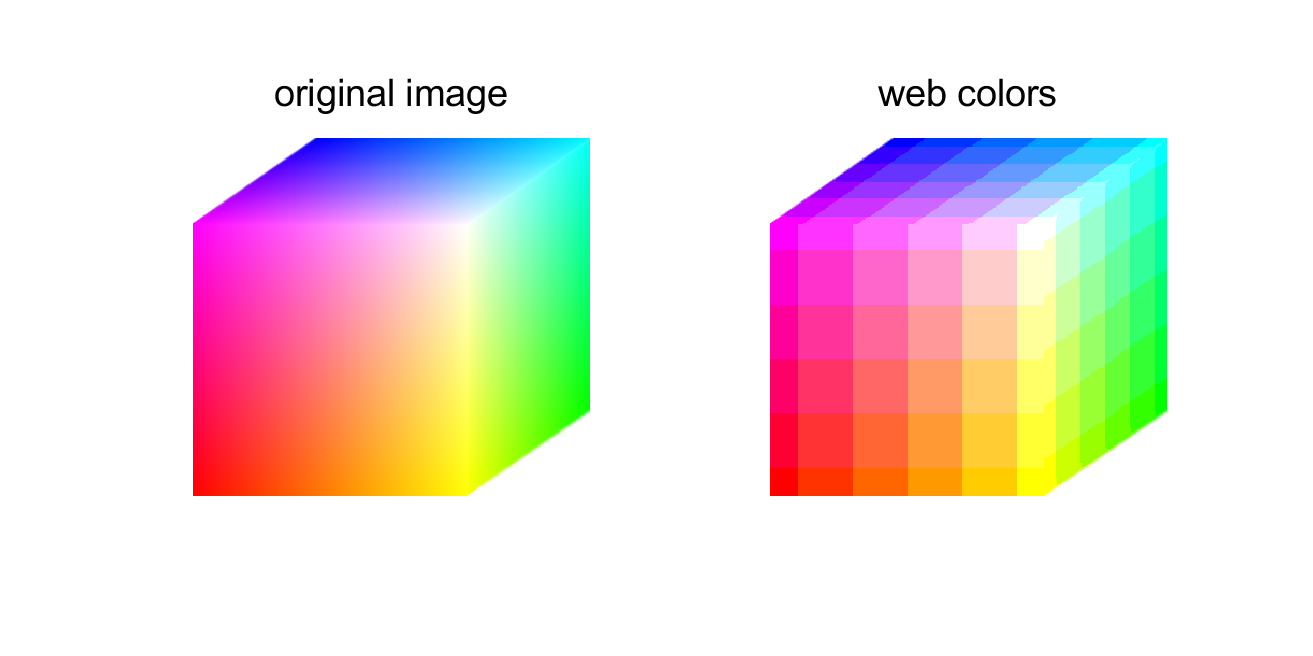
\includegraphics[width = 0.6\textwidth]{第三次/f1.png}
            \caption{实验结果}
        \end{figure}

        可以看到原图为24bit的立方体,经过处理之后其颜色总数变少,理论上只有$6^3 = 216$个。

    \section{总结}
    本次实验主要是通过Matlab编程语言实现了课程中所讲过的网页安全色。

    同时也对RBG色彩模式的图像处理有了更加深刻的理解。

\end{document}



